


\tikzset{every picture/.style={line width=0.75pt}} %set default line width to 0.75pt        

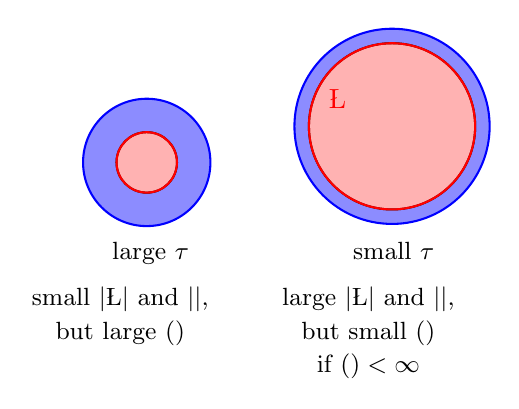
\begin{tikzpicture}[x=0.75pt,y=0.75pt,yscale=-1,xscale=1,scale=0.9]
%uncomment if require: \path (0,797); %set diagram left start at 0, and has height of 797

%Shape: Circle [id:dp4134875770594737] 
\draw  [color={rgb, 255:red, 0; green, 0; blue, 255 }  ,draw opacity=1 ][fill={rgb, 255:red, 0; green, 0; blue, 255 }  ,fill opacity=0.45 ] (262.25,535.5) .. controls (262.25,506.64) and (285.64,483.25) .. (314.5,483.25) .. controls (343.36,483.25) and (366.75,506.64) .. (366.75,535.5) .. controls (366.75,564.36) and (343.36,587.75) .. (314.5,587.75) .. controls (285.64,587.75) and (262.25,564.36) .. (262.25,535.5) -- cycle ;
%Shape: Circle [id:dp3677137074190848] 
\draw  [fill={rgb, 255:red, 255; green, 255; blue, 255 }  ,fill opacity=1 ] (270,535.5) .. controls (270,510.92) and (289.92,491) .. (314.5,491) .. controls (339.08,491) and (359,510.92) .. (359,535.5) .. controls (359,560.08) and (339.08,580) .. (314.5,580) .. controls (289.92,580) and (270,560.08) .. (270,535.5) -- cycle ;
%Shape: Circle [id:dp29158884164216103] 
\draw  [color={rgb, 255:red, 255; green, 0; blue, 0 }  ,draw opacity=1 ][fill={rgb, 255:red, 255; green, 0; blue, 0 }  ,fill opacity=0.3 ] (270,535.5) .. controls (270,510.92) and (289.92,491) .. (314.5,491) .. controls (339.08,491) and (359,510.92) .. (359,535.5) .. controls (359,560.08) and (339.08,580) .. (314.5,580) .. controls (289.92,580) and (270,560.08) .. (270,535.5) -- cycle ;
%Shape: Circle [id:dp7745915065874394] 
\draw  [color={rgb, 255:red, 0; green, 0; blue, 255 }  ,draw opacity=1 ][fill={rgb, 255:red, 0; green, 0; blue, 255 }  ,fill opacity=0.45 ] (149.09,554.82) .. controls (149.09,535.99) and (164.35,520.73) .. (183.18,520.73) .. controls (202.01,520.73) and (217.27,535.99) .. (217.27,554.82) .. controls (217.27,573.65) and (202.01,588.91) .. (183.18,588.91) .. controls (164.35,588.91) and (149.09,573.65) .. (149.09,554.82) -- cycle ;
%Shape: Circle [id:dp8874236690779891] 
\draw  [fill={rgb, 255:red, 255; green, 255; blue, 255 }  ,fill opacity=1 ] (167,554.82) .. controls (167,545.88) and (174.25,538.63) .. (183.18,538.63) .. controls (192.12,538.63) and (199.37,545.88) .. (199.37,554.82) .. controls (199.37,563.75) and (192.12,571) .. (183.18,571) .. controls (174.25,571) and (167,563.75) .. (167,554.82) -- cycle ;
%Shape: Circle [id:dp9801257697618313] 
\draw  [color={rgb, 255:red, 255; green, 0; blue, 0 }  ,draw opacity=1 ][fill={rgb, 255:red, 255; green, 0; blue, 0 }  ,fill opacity=0.3 ] (167,554.82) .. controls (167,545.88) and (174.25,538.63) .. (183.18,538.63) .. controls (192.12,538.63) and (199.37,545.88) .. (199.37,554.82) .. controls (199.37,563.75) and (192.12,571) .. (183.18,571) .. controls (174.25,571) and (167,563.75) .. (167,554.82) -- cycle ;


% Text Node
\draw (279,514) node [anchor=north west][inner sep=0.75pt]  [color={rgb, 255:red, 255; green, 0; blue, 0 }  ,opacity=1 ]  {$\L$};
% Text Node
\draw (246,496) node [anchor=north west][inner sep=0.75pt]  [color={rgb, 255:red, 0; green, 0; blue, 255 }  ,opacity=1 ]  {\U};
% Text Node
\draw (163,596) node [anchor=north west][inner sep=0.75pt]   [align=left] {\small large $\displaystyle \tau $};
% Text Node
\onslide<6->{\draw (120,620) node [anchor=north west][inner sep=0.75pt]   [align=center] {\small small $|\L|$ and $|\U|$,\\\small but large $\w(\U)$};}
% Text Node
\draw (292,596) node [anchor=north west][inner sep=0.75pt]   [align=left] {\small small $\displaystyle \tau $};
% Text Node
\onslide<7->{\draw (254,620) node [anchor=north west][inner sep=0.75pt]   [align=center] {\small large $|\L|$ and $|\U|$,\\\small but small $\w(\U)$ \\\small if $\w(\C) < \infty$};}


\end{tikzpicture}
